%%%%%%%%%%%%%%%%%%%%%%%%%%%%%%%%%%%%%%%%%
% baposter Landscape Poster
% LaTeX Template
% Version 1.0 (11/06/13)
%
% baposter Class Created by:
% Brian Amberg (baposter@brian-amberg.de)
%
% This template has been downloaded from:
% http://www.LaTeXTemplates.com
%
% License:
% CC BY-NC-SA 3.0 (http://creativecommons.org/licenses/by-nc-sa/3.0/)
%
%%%%%%%%%%%%%%%%%%%%%%%%%%%%%%%%%%%%%%%%%

%-------------------------------------------------------------------------------------
%	PACKAGES AND OTHER DOCUMENT CONFIGURATIONS
%-------------------------------------------------------------------------------------

\documentclass[landscape,a0paper,fontscale=0.285]{baposter} % Adjust the font scale/size here

\usepackage{graphicx} % Required for including images
\graphicspath{{figures/}} % Directory in which figures are stored

\usepackage{amsmath} % For typesetting math
\usepackage{amssymb} % Adds new symbols to be used in math mode

\usepackage{booktabs} % Top and bottom rules for tables
\usepackage{enumitem} % Used to reduce itemize/enumerate spacing
\usepackage{palatino} % Use the Palatino font
\usepackage[font=small,labelfont=bf]{caption} % Required for specifying captions to tables and figures

\usepackage{multicol} % Required for multiple columns
\setlength{\columnsep}{1.5em} % Slightly increase the space between columns
\setlength{\columnseprule}{0mm} % No horizontal rule between columns

\usepackage{tikz} % Required for flow chart
\usetikzlibrary{shapes,arrows} 
    % Tikz libraries required for the flow chart in the template

%% Other packages needed for the poster
\usepackage{enumitem}

\newcommand{\compresslist}{ % Define a command to reduce spacing within itemize/enumerate environments, this is used right after \begin{itemize} or \begin{enumerate}
\setlength{\itemsep}{1pt}
\setlength{\parskip}{0pt}
\setlength{\parsep}{0pt}
}

\definecolor{lightblue}{rgb}{0.145,0.6666,1} 
      % Defines the color used for content box headers

%%% Other colors needed for the poster.
%%%
\definecolor{olive}{rgb}{0.3, 0.4, .1}
\definecolor{fore}{RGB}{249,242,215}
\definecolor{back}{RGB}{51,51,51}
\definecolor{title}{RGB}{255,0,90}
\definecolor{dgreen}{rgb}{0.,0.6,0.}
\definecolor{gold}{rgb}{1.,0.84,0.}
\definecolor{JungleGreen}{cmyk}{0.99,0,0.52,0}
\definecolor{BlueGreen}{cmyk}{0.85,0,0.33,0}
\definecolor{RawSienna}{cmyk}{0,0.72,1,0.45}
\definecolor{Magenta}{cmyk}{0,1,0,0}
%%%

%%% Symbols needed for dynamical system definitions.
%%%
\newcommand{\cals}{\mbox{$\mathcal{S}$}}
\newcommand{\calc}{\mbox{$\mathcal{C}$}}
\newcommand{\calcp}{\mbox{$\mathcal{C'}$}}

\newcommand{\bbb}{\mbox{$\mathbb{B}$}}
\newcommand{\cala}{\mbox{$\mathcal{A}$}}
\newcommand{\calcdp}{\mbox{$\mathcal{C}^{''}$}}
\newcommand{\calco}{\mbox{$\mathcal{C}_1$}}
\newcommand{\calct}{\mbox{$\mathcal{C}_2$}}
\newcommand{\calcv}{\mbox{$\mathcal{C}_v$}}
\newcommand{\calf}{\mbox{$\mathcal{F}$}}
\newcommand{\calp}{\mbox{$\mathcal{P}$}}
\newcommand{\calso}{\mbox{$\mathcal{S}_1$}}

\newcommand{\cpsp}{\mbox{\textbf{PSPACE}}}
\newcommand{\ccnp}{\mbox{\textbf{Co-NP}}}
%%%


\begin{document}

\begin{poster}
{
headerborder=closed, % Adds a border around the header of content boxes
colspacing=1em, % Column spacing
bgColorOne=white, % Background color for the gradient on the left side of the poster
bgColorTwo=white, % Background color for the gradient on the right side of the poster
borderColor=lightblue, % Border color
headerColorOne=black, % Background color for the header in the content boxes (left side)
headerColorTwo=lightblue, % Background color for the header in the content boxes (right side)
headerFontColor=white, % Text color for the header text in the content boxes
boxColorOne=white, % Background color of the content boxes
textborder=roundedleft, % Format of the border around content boxes, can be: none, bars, coils, triangles, rectangle, rounded, roundedsmall, roundedright or faded
eyecatcher=true, % Set to false for ignoring the left logo in the title and move the title left
headerheight=0.19\textheight, % Height of the header
headershape=roundedright, % Specify the rounded corner in the content box headers, can be: rectangle, small-rounded, roundedright, roundedleft or rounded
headerfont=\Large\bf\textsc, % Large, bold and sans serif font in the headers of content boxes
%textfont={\setlength{\parindent}{1.5em}}, % Uncomment for paragraph indentation
linewidth=2pt % Width of the border lines around content boxes
}
%----------------------------------------------------------------------------------------
%	TITLE SECTION 
%----------------------------------------------------------------------------------------
%
{
\includegraphics[height=6em]{uva_logo.png}} % First university/lab logo on the left
{\textbf{Synchronous Dynamical Systems on Directed Acyclic Graphs (DAGs):
            Complexity and Algorithms}\vspace{0.25em}
} % Poster title
{\textcolor{green}{\textbf{Daniel J. Rosenkrantz$\,{}^{1,2}$,~ 
         Madhav V. Marathe$\,{}^1$,~ S. S. Ravi$\,{}^{1,2}$,~
         Richard E. Stearns$\,{}^{1,2}$}}\\ \vspace{0.1em} 
            {$^1$University of Virginia~ and~
            $^2$University at Albany -- State University 
            of New York} \\ \vspace{0.25em}
            \textcolor{magenta}{
               \textbf{(Poster Presented at  AAAI-2021)}}
            } % Author names and institution
{
\includegraphics[height=8em]{ualbany_logo.png}} 
             % Second university/lab logo on the right
%------------------------------------------------------------------------------------
%	BASICS OF SYDSs
%------------------------------------------------------------------------------------

\headerbox{Dynamical Systems: Basics}
          {name=SyDSBasics,column=0,row=0}{
A \textcolor{magenta}{
\textbf{Discrete Dynamical System on a DAG}} ~\cals{} has:

\smallskip

\begin{itemize}[leftmargin=*,noitemsep,topsep=0pt]
\compresslist
\item An underlying DAG $G(V,E)$.  
\item \textbf{Nodes:}~ Agents in the system. 
\item \textbf{Edges:}~ Permissible local interactions.  
\item State values for nodes from a finite\newline domain \bbb{}.
      (Here, \textcolor{dgreen}{\textbf{\bbb{} = \{0,~1\}}}.) 
\item A \textbf{local transition function} for each node.
\item \textbf{Update mechanism:} \textcolor{magenta}{\textbf{synchronous}}.
\end{itemize}

\medskip

\noindent
\textbf{Notation:}~ DAG-SyDS~ (Synchronous\newline Dynamical System on a DAG)

\medskip

\noindent
\textcolor{green}{\textbf{Local Transition Function:}}

\medskip

\begin{minipage}{0.25\textwidth}
\begin{center}
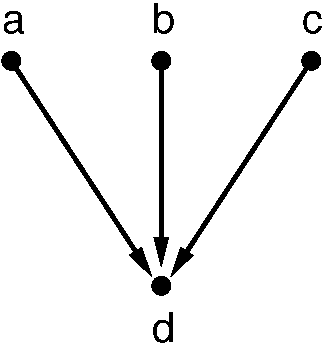
\includegraphics[scale=0.35]{local_function.pdf}
\end{center}
\end{minipage}
\hspace*{0.2in}
\begin{minipage}{0.6\textwidth}
\textbf{Local function}~ $f_d\:$:

%\medskip

\begin{itemize}[leftmargin=*,noitemsep,topsep=0pt]\compresslist
\item \underline{Inputs:}~
States of $a$, $b$, $c$\\ and $d$.  
\item \underline{Output:}~ Next state of $d$.
\end{itemize}
\end{minipage}

%\bigskip\bigskip
\medskip

\begin{itemize}[leftmargin=*,noitemsep,topsep=0pt]\compresslist
\item The only input to the local function $f_a$ is\newline
the state of $a$. %\\ \medskip
\item A similar comment applies to the local\newline functions
$f_b$ and $f_c$.
\end{itemize}

\medskip

\noindent
\textbf{Note:}~ The local functions are 
\textcolor{magenta}{\textbf{deterministic}}.
}

%------------------------------------------------------------------------------------
%	EXAMPLES
%------------------------------------------------------------------------------------

\headerbox{Examples}{name=examples,row=0,column=1}{

\textcolor{green}{\textbf{DAG-SyDS Example:}}

\medskip

\begin{minipage}{0.4\textwidth}
\begin{center}
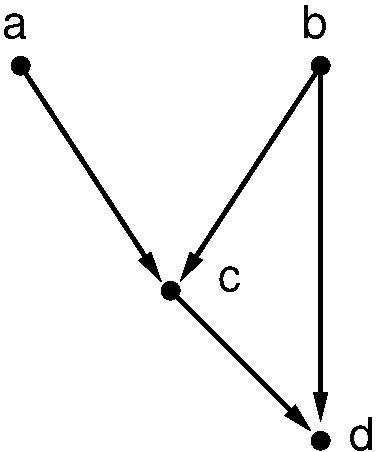
\includegraphics[scale=0.30]{dag_syds_example.pdf}
\end{center}
\end{minipage}
\quad
\begin{minipage}{0.5\textwidth}
\begin{itemize}[leftmargin=*,noitemsep,topsep=0pt]\compresslist
\item $\bbb$ = $\{0,1\}$ %\medskip
\item $f_a\:$:~ Zero function %\medskip
\item $f_b\:$:~ Identity function %\medskip
\item $f_c\:$:~ OR function %\medskip
\item $f_d\:$:~ AND function
\end{itemize}
\end{minipage}

\bigskip

\textcolor{green}{\textbf{Time Evolution of the Above DAG-SyDS:}}
\begin{center}
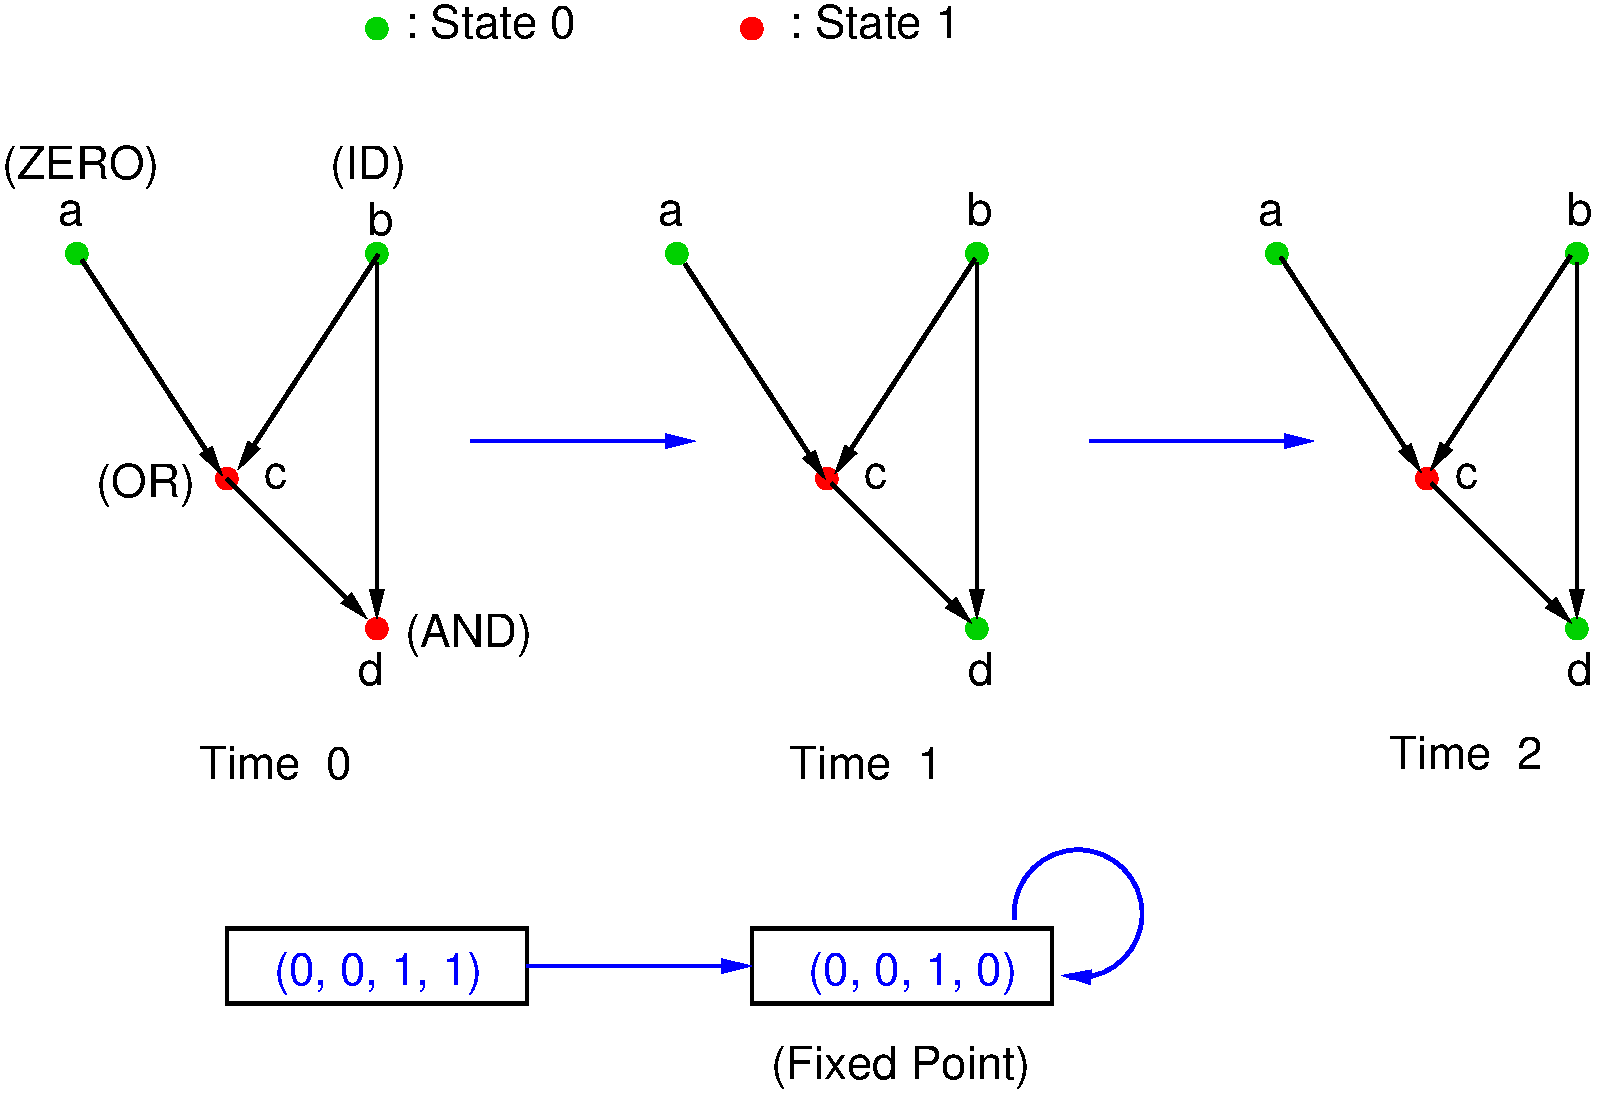
\includegraphics[scale=0.25]{time_evolution.pdf}
\end{center}
}

%------------------------------------------------------------------------------------
%	Some Defs. + Phase Space
%------------------------------------------------------------------------------------

\headerbox{Definitions}{name=SomeDefs,row=0,column=2}{
\small{
\begin{itemize}[leftmargin=*,noitemsep,topsep=0pt]
\compresslist
\item \textcolor{magenta}{\textbf{Configuration}} at time $t$:~ Vector specifying
the state of each node at time $t$.  %\medskip

\item \textcolor{magenta}{\textbf{Successor}} of a configuration \calc:~ 
The configuration
that \textbf{immediately follows} \calc{}
in time evolution. %\medskip

\item \textcolor{magenta}{\textbf{Fixed Point}}:~
A configuration \calc{} whose successor\newline is \calc{} itself. %\bigskip
%\medskip

\item The \textcolor{magenta}{\textbf{phase space}} of a
discrete dynamical system \cals{} is a 
\textbf{directed graph} \calp.  %\smallskip
  \begin{itemize}[leftmargin=*,noitemsep,topsep=0pt]\compresslist
    \item Each node of \calp{} represents a configuration of \cals.  %\smallskip
    \item Each directed edge $(x,y)$ indicates that $y$ is the successor of $x$.
  \end{itemize}
\end{itemize}
\medskip
\textbf{Note:}~ The
size of \calp{} is \textcolor{red}{\textbf{exponential}} in the size of \cals.
}

\medskip

\textcolor{green}{\textbf{Example -- Phase Space of DAG-SyDS \cals:}}

\begin{center}
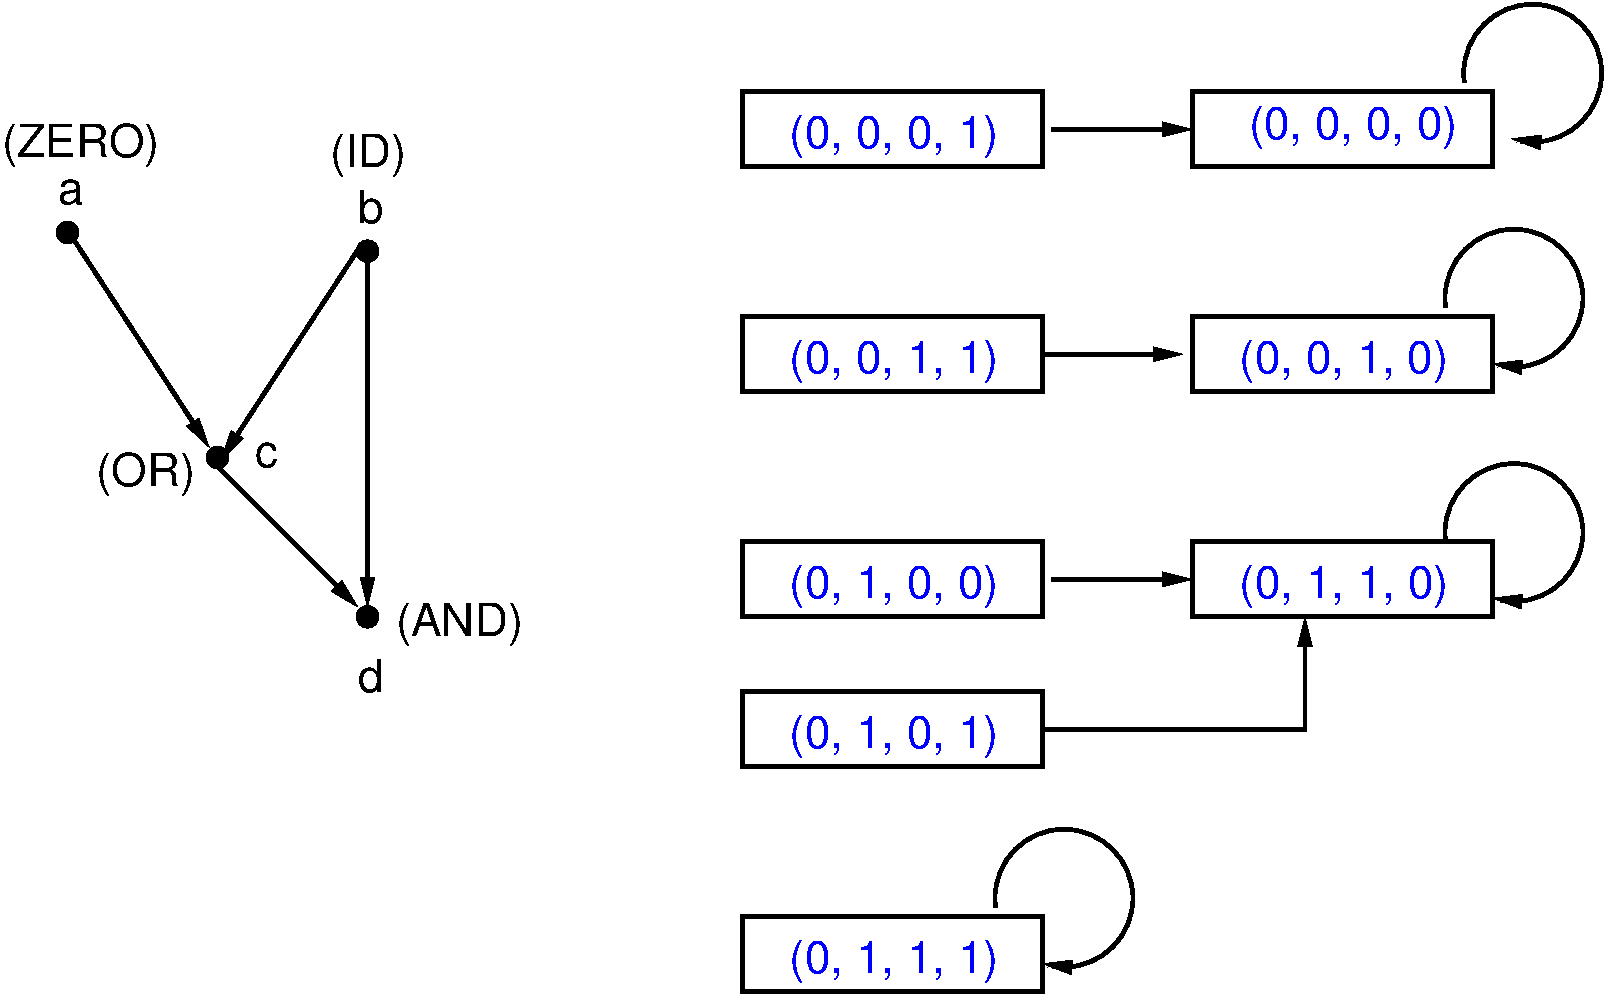
\includegraphics[scale=0.25]{phase_space.pdf}
\end{center}
%\smallskip
\small{\textbf{Note:}~ Only a part of the phase space is shown.}
}

%------------------------------------------------------------------------------------
%       Problems Considered
%------------------------------------------------------------------------------------

\headerbox{Problems Considered}{name=Problems,row=0,column=3}{

\textcolor{green}{\textbf{Motivation -- Diffusion in Networks:}}

{\small
\begin{itemize}[leftmargin=*,noitemsep,topsep=0pt]
\compresslist
\item \textcolor{magenta}{\textbf{Contagion}} processes model many social phenomena \\
      (e.g., propagation of information, influence,
      diseases, trends, etc.). %\medskip
\item Example: Diffusion of opinions in networks
(e.g., \textcolor{blue}{[Auletta et al. 2018, 
Chistikov et al. 2020, Botan et al. 2019, Bredereck \& Elkind 2017]}).
%\medskip
\item Usual modeling assumptions:
    \begin{itemize}[leftmargin=*,noitemsep,topsep=0pt]
    \compresslist
        \item Agents in the system have states that vary\newline with time. %\medskip
        \item The next state of an agent depends on her current state
              and those of her neighbors (i.e.,
              agent\newline interactions are \textcolor{magenta}{\textbf{local}}).
     \end{itemize}
\smallskip
%\item \textcolor{magenta}{\textbf{Threshold-based}} mechanisms commonly used to capture
%     behavior; the behavior of an agent depends
%     on how many of its neighbors are in certain states (e.g.,
%     \textcolor{blue}{[Granovetter~1978, Easley \& Kleinberg~2010]}).

%\medskip
%\item \textcolor{magenta}{\textbf{Discrete Dynamical Systems:}}~ A formal model for
%analyzing contagion phenomena.
\end{itemize}
}
%\vspace*{-2in}
\textcolor{green}{\textbf{Analysis Problems:}}

\smallskip

\textcolor{magenta}{\textbf{Reachability:}} \smallskip

\noindent
\textbf{Given:}~ SyDS $S$ and
configurations \calco{} and \calct.  %\smallskip

\textbf{Question:}~ Does \cals{} starting from \calco{} 
reach \calct?

\smallskip

\textcolor{magenta}{\textbf{Convergence:}} \smallskip

\noindent
\textbf{Given:}~ SyDS $S$ and
configuration \calco. %\smallskip

\noindent
\textbf{Question:}~ Does \cals{} starting from \calco{} 
reach a\newline fixed point?

\smallskip

\textcolor{magenta}{\textbf{Convergence Guarantee:}} \smallskip

\noindent
\textbf{Given:}~ SyDS $S$.  %\smallskip

\textbf{Question:}~ Does \cals{} reach a fixed point
from\newline \textcolor{red}{\textbf{every}} starting configuration?

\smallskip

\textcolor{blue}{\textbf{Note:}~ The above questions concern
the\newline phase space $\calp(\cals)$ of \cals.}
}

%------------------------------------------------------------------------------------
%       Some Previous Work
%------------------------------------------------------------------------------------

\headerbox{Previous Work (Brief)}{name=PrevWork,row=1,below=SyDSBasics}{

\begin{itemize}[leftmargin=*,noitemsep,topsep=0pt]
\compresslist
\item Hardness of Reachability and 
Convergence for undirected graphs
(e.g., \textcolor{blue}{[Barrett et al. 2006, Rosenkrantz et al. 2018]}).
%\medskip
\item Hardness results for directed graphs 
\textcolor{blue}{[Ogihara \& Uchizawa: 2017 \& 2020]}. %\medskip
\item Hardness results for Hopfield neural nets (e.g., 
         \textcolor{blue}{[Orponen 1994]}) and Petri nets 
         (e.g., \textcolor{blue}{[Esparza \& Nielsen 1994]}).
\item Efficient algorithm for Reachability for DAG-SyDSs with 
\textcolor{magenta}{\textbf{bi-threshold}} functions
(\textcolor{blue}{[Kuhlman et al. 2013]}).
\item Efficient algorithm for  controlling a SyDS 
on a \textcolor{dgreen}{\textbf{directed tree}}
so that it reaches a desirable\newline configuration 
(\textcolor{blue}{[Akutsu et al. 2007]}).
\end{itemize}
}

%------------------------------------------------------------------------------------
%       Chistikov et al. (AAAI 2020)
%------------------------------------------------------------------------------------

\headerbox{Chistikov et al. \small{(AAAI-2020)}}
          {name=Chistikov,row=1,column=1,below=examples}{
{\small
\begin{itemize}[leftmargin=*,noitemsep,topsep=0pt]
\compresslist
\item SyDSs on directed graphs in the context of diffusion
of opinions. \smallskip
\item Each local function is the \textcolor{magenta}{\textbf{majority}}
function: an agent changes her \{0,1\} opinion only when a majority
of her neighbors have a different opinion.\smallskip
%(This function is 2-symmetric.) \medskip
\item The Convergence problem is efficiently solvable for DAG-SyDSs
regardless of local functions. \smallskip
\item Convergence and Convergence Guarantee problems are
\cpsp-complete for SyDSs on directed graphs where each local
function is the majority function. %\medskip
\end{itemize}
}
}

%------------------------------------------------------------------------------------
%       Our Contributions -- I
%------------------------------------------------------------------------------------

\headerbox{Our Contributions -- I}
          {name=MainContrib,row=1,column=2,below=SomeDefs}{
{\small
\begin{itemize}[leftmargin=*,noitemsep,topsep=0pt]\compresslist
\item \textcolor{blue}{Reachability} is \cpsp-complete 
for \textcolor{magenta}{\textbf{symmetric}} DAG-SyDSs.\smallskip

\textbf{Proof Idea:}~ Reduction from Quantified 3SAT.

\item \textcolor{blue}{Convergence Guarantee} is  \ccnp-complete
for DAG-SyDSs with at most \textcolor{dgreen}{\textbf{three}} levels.
\smallskip

\textbf{Proof Idea:}~ Reduction from 3SAT.\smallskip

\item New structural properties of the phase spaces of DAG-SyDSs
(e.g., bounds on lengths of cycles and transients in phase space).
\end{itemize}
}
}

%------------------------------------------------------------------------------------
%       Our Contributions -- II
%------------------------------------------------------------------------------------

\headerbox{Our Contributions -- II}
          {name=MainContrib-II,row=1,column=3,below=Problems}{

\begin{itemize}[leftmargin=*,noitemsep,topsep=0pt]\compresslist
\item \textcolor{blue}{Reachability} is  efficiently solvable
for\newline \textcolor{magenta}{\textbf{monotone}} DAG-SyDSs. \smallskip

\textbf{Proof Idea:}~ Show that each cycle is a fixed point; 
use the result that the transient length is $\leq$
the number of levels in the DAG.
\end{itemize}

\medskip

\textcolor{green}{\textbf{Future Work:}} \smallskip

\begin{itemize}[leftmargin=*,noitemsep,topsep=0pt]\compresslist
\item DAG-SyDSs with other
local functions\newline (e.g., weighted threshold functions). %\bigskip

%\item  Restricted forms of DAGs (e.g., bounded indegree). %\bigskip

\item Stochastic DAG-SyDSs.
\end{itemize}
}

%------------------------------------------------------------------------------------
%       Acknowledgments
%------------------------------------------------------------------------------------

\headerbox{Acknowledgments}
          {name=Ack,row=2,column=1,below=Chistikov}{
{\small 
We thank the referees of AAAI-2021 for providing
helpful feedback. 
This work was partially supported by NSF
Grants IIS-1633028 (BIG DATA), CMMI-1745207 (EAGER), OAC-1916805
(CINES), CCF-1918656 (Expeditions) and IIS-1908530.}
}

%------------------------------------------------------------------------------------
%       Contact Author
%------------------------------------------------------------------------------------

\headerbox{Contact Author}
          {name=Contact,row=2,column=2,below=MainContrib}{
{S. S. Ravi~ (\textcolor{green}{\textbf{\texttt{ssravi0@gmail.com}}})}
}

\end{poster}

\end{document}
